\section{Introduction}


\begin{frame}{Pulsar Glitches}
	
	\begin{minipage}{0.53\textwidth}
		\textbf{Pulsars}: rapidly rotating, highly magnetized neutron stars that slowly spin down. Occasionally, they exhibit sudden spin-up events called \textbf{glitches}.
		
	\end{minipage}%
	\begin{minipage}{0.46\textwidth}
		\centering
		\vspace{1em}
		\begin{figure}
			\centering
			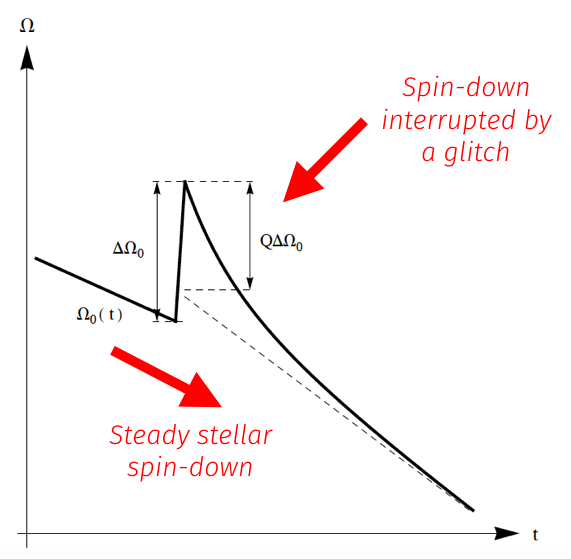
\includegraphics[width=0.8\linewidth]{assets/glitch.png}
			
			\vspace{-0.5em}
			
			\caption{\footnotesize Glitch and spin-down \cite{vanEysden2011}}
		\end{figure}
	\end{minipage}

	\vspace{-1em}

	Glitches likely result from:
	
		\begin{itemize}
			\item sudden unpinning of superfluid vortices
			\item crustal failures
		\end{itemize}

	Both release stored angular momentum, causing the spin-up.

\end{frame}


\begin{frame}{Role of Stochastic Processes}

	Stochastic processes can be used to model glitches in a microphysics-agnostic approach.

	In particular:

	\vspace{0.2cm}
	{
	\setlength{\leftmargini}{1.5em}
	\setlength{\leftmarginii}{1.2em}
	\begin{itemize}
		\item \textbf{Brownian Process} \footnotesize - \textit{Carlin \& Melatos (2020)} \cite{CarlinMelatos2020}
		\normalsize
		\begin{itemize}
			\item Internal stress builds up stochastically as a Brownian process between glitch events.
			\vspace{0.2cm}
			\item A glitch occurs when the stress exceeds a critical \textbf{\textit{threshold}}.
		\end{itemize}
		\vspace{0.3cm}
		\item \textbf{State-dependent Poisson Process} \footnotesize - \textit{Fulgenzi, \& Melatos (2017)} \cite{FulgenziMelatosHughes2017}
		\normalsize
		\begin{itemize}
			\item The glitch rate is a function of the stress.
			\vspace{0.2cm}
			\item The stress increases linearly between glitch events.
		\end{itemize}
	\end{itemize}
	}
	
\end{frame}





